\chapter{Segmentation} \label{ch:segmentation}

We discuss how we use the Frangi as a prefilter and discuss several different segmentation strategies based upon our Frangi-filtered result. We will compare these methods to an unrelated segmentation strategy, the ISODATA threshold. First, we define some standard quantitative measures of success for segmentation methods.


\subsection{Binary classifications and the confusion matrix}

We wish to come up wish a means of gauging the success of an arbitrary segmentation and will adopt a binary classification model to do so.
We end up with a boolean matrix the size of the image, and compare it to the ground truth, the trace, and then compare them to get the number of true positives (TP), true negatives (TN), false positives (FP), and false negatives (FN). We demonstrate these four labels visually with a confusion matrix, as in \cref{fig:sample-confusion}. The lighter gray represents true negatives (TN), red represents false negatives (FN), blue represents false positives (FP), and black represents true positives. The darkest gray are is the background mask (pixels are not considered at all in gauging the success of segmentation).
 
\begin{figure}
  \centering
  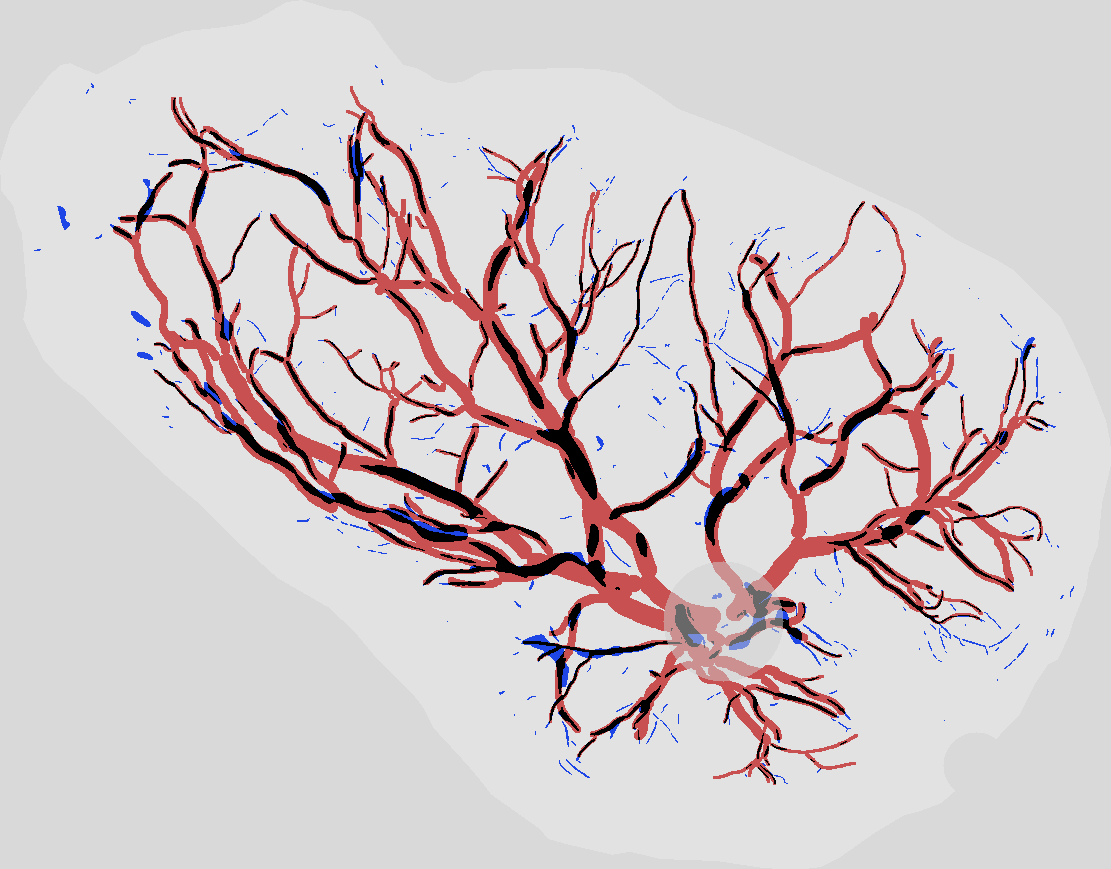
\includegraphics[width=0.5\textwidth]{sample_confusion}
  \caption{Sample confusion matrix}
  \label{fig:sample-confusion}
\end{figure}

Although there are many measures to gauge the success of binary classification, we will focus on two that we find particularly illustrative. The first is precision, given by

\begin{equation}
\label{eq:precision}
\textrm{precision} \;=\; \frac{TP}{TP+FP}
\end{equation}

and the second is the Matthews Correlation Constant (MCC), given by

\begin{equation} \label{eq:MCC}
MCC = \frac{TP\times TN - FP \times FN}{\sqrt{ (TP + FP)(TP+FN)(TN+FP)(TN+FN)}}
\end{equation}

where precision is a ratio between 0 \% and 100\% and the MCC is a measure between -1 and 1. Precision (or positive predictive power) is of course a ratio between how many pixels were labeled correctly and all pixels labeled positive (correctly or incorrectly). This is a useful score for us--if we are using Frangi as a prefiltering for a more robust technique, we would not want to provide any wrong information or seeds to that algorithm. Precision therefore does an okay job of representing that scenario: we are not penalized for what we do not label as true, as long as our reports of true are correct.

Of course, we cannot rely on precision as our sole quantiative factor alone--we could simply return everything negative and recieve a perfect score of 100\% precision. Therefore we will gauge that measure with that of the MCC \cite{mcc-original-paper}. The main advantage of the MCC is that it is well balanced no matter what the size of the two classes are, and will only be high if the approximation scores well against both labels. A score of $1.0$ means the approximation is 100\% correct, a score of $-1.0$ means that everything is completely incorrect, and a score of $0$ means that the test performs only as well as random guessing. In our analysis, we will consider both the MCC and precision of a particular segmentation simultaneously. We would like an MCC score as high as possible, but will contextually settle for a lower score as long as the approximation is still \textit{precise}.

One final point about these measures is that we have decided to report their scores only within the placental plate, rather than the entire rectangular image. Since the area outside of plate is masked from consideration, those points will be true negatives no matter what, and we don't want this artificial padding to influence our score. That being said, we do currently concede one part right now: we will also mask an area around the umbilical cord insertion point, as the large amount of noise here will mean that our scores are artificially low. We would like to remove these areas, but for now we will simply not score them. 

\section{Postprocessing Techniques}
Here we develop four relatively straightforward methods of postprocessing the multiscale Frangi output to obtain an actual PCSVN extraction. Again, we stress that the Frangi filter itself does not produce a segmentation itself. In fact, Frangi in his original paper \cite{frangi-paper} refrained from any explicit analysis of the Frangi score apart from taking the maximum across all scales. Still, we wish to demonstrate some immediate methods of postprocessing these samples in order to illustrate the usefulness of this optimized Frangi filter. 



\subsection{Method A: Fixed Threshold}

In the fixed threshold method, we choose some threshold $\alpha$ and we say that a pixel $(x,y)$ of the image corresponds to a vessel if
$\Vmax >  \alpha$. This $\alpha$, as noted above, is unfortunately highly dependent on the image domain, and this merging method will tend to happily allow noise generated from scales that are too large or too small.
 Another issue with this is the individual scales of the Frangi filter in the extreme cases are not known to scale--although Lindeberg introduced a normalization factor based on the scale to apply to the derivatives, we do not know of an optimal factor to use.

Unfortunately, even with our ``rescaled'' Frangi filter, this $\alpha$ cannot be picked without regard for the particular image domain. Equally problematic, we cannot guarantee that the Frangi filter will decay as our scale exceeds the the bounds where structure is expected to be found. Ideally we could create a filter that would do that.

 Nonetheless, we wish to demonstrate the usefulness of the Frangi filter within our image domain towards the segmentation problem, and will therefore, like \cite{huynh2013filter}, consider a thresholded \Vmax{} as a crude segmentation. 
\begin{equation}
{\VSigma}_{\alpha}(x_0,y_0) = \begin{cases}
1 & \textrm{if}\quad \Vmax(x,y) \; \ge\;  \alpha \\
0 & \textrm{else}
\end{cases}  \quad , \; \alpha > 0
\; \textrm{for}\;\alpha\;\textrm{fixed}.
\end{equation}

If we insist on such a performing such a thresholding, the ``correct'' choice of $\alpha$ unfortunately seems to depend on the image domain, so user intervention when dealing with the problem domain seems to be the best strategy. A more sincere use of thresholding might be to choose a relatively high threshold, and then use the result for a further technique.
We will discuss alternatives methods of aggregating results from our multiscale method, as well as optimal values for parameters and scales. As a final note, we admit that any future extensions of this work (as will be discussed in \cref{ch:conclusion}) should not hold too much stock in this thresholded result, and analyzing the 
raw vesselness score \cref{eq:Vmax}, or even the un-merged scale-wise scores, would be far more rewarding.    
\subsection{Method B: Percentile Based Merging}

The idea behind percentile-based merging is beneficial for large multiscale methods. At each scale, we would like to assume that there is \textit{some} curvilinear content that could be identified. With that in mind, we could simply accept from each scales scores in a very high percentile. We chose for our demonstration a fairly large percentile, $95$, and furthermore bolster this by requiring that any selected pixels be in the 95th percentile of nonzero and unmasked pixels--otherwise the average is artificially low due to the large background and pixels with zero Frangi score. The use of percentiles removes dependence of picking a particular threshold on the problem, while allowing the most prominent features to emerge at each scale, but of course it unfortunately treats all scales equally, so the success of the multiscale approach here is very dependent on choice of $\sigma_{\min}$ and $\sigma_{\max}$.

	We briefly demonstrate this in \cref{fig:qthresh_demo} on a particularly well-behaved sample. The top left value image is the original (grayscale image), the top right is $\Vmax$, the bottom left is the 95th percentile of nonzero scores of each scale, and the bottom right is the 98th percentile of nonzero scores at each scale.

\begin{figure} \centering
  \subfloat{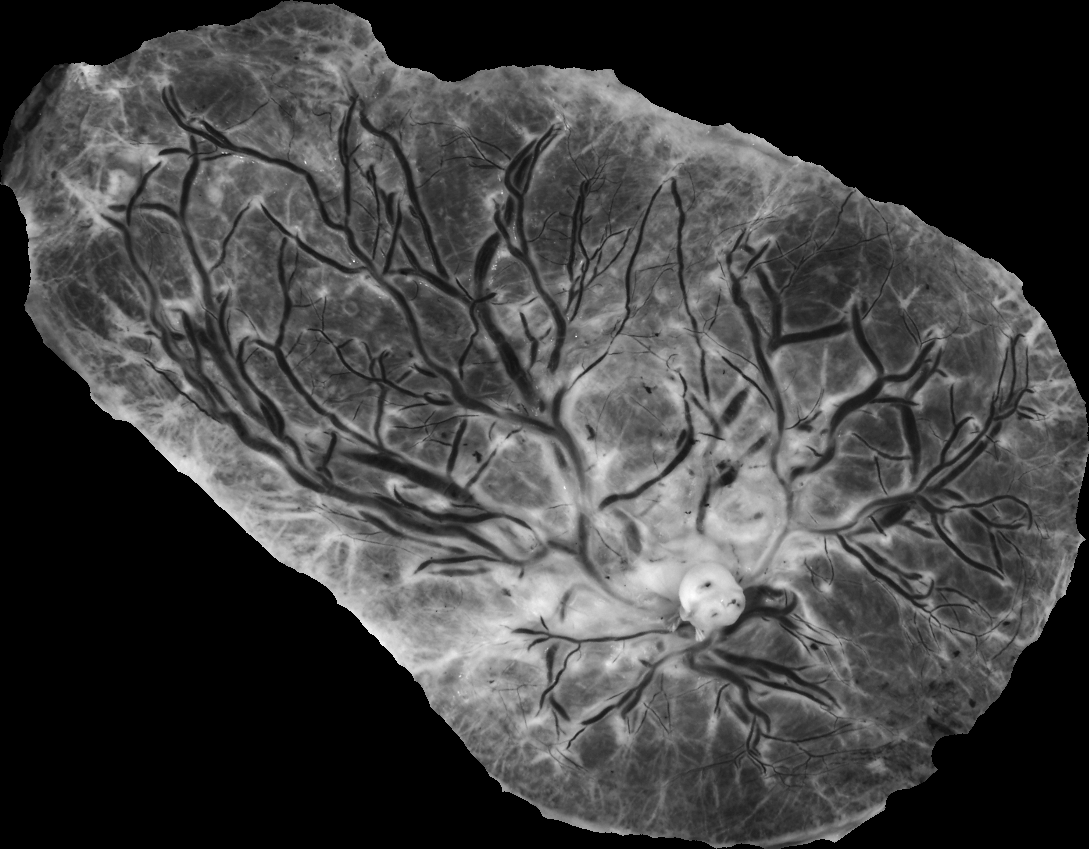
\includegraphics[width=0.48\linewidth]{qthresh_demo_img}} \;
  \subfloat{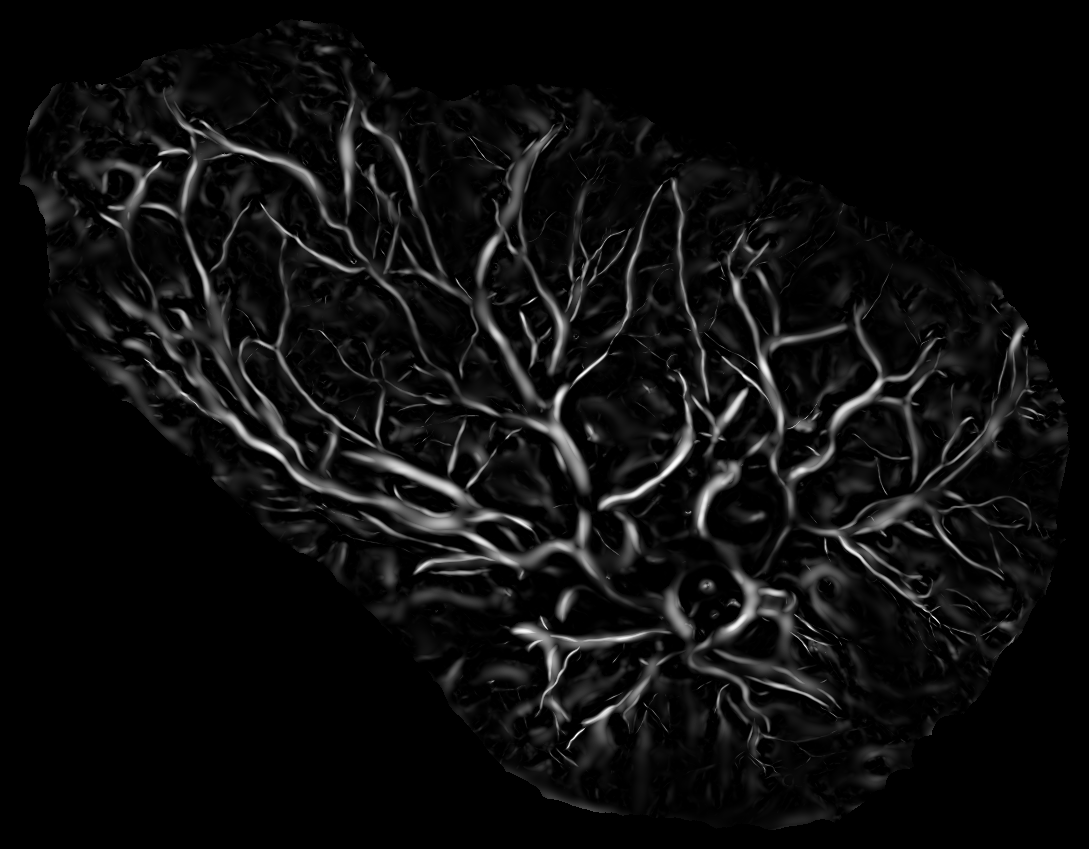
\includegraphics[width=0.48\linewidth]{qthresh_demo_Fmax}} \\
  \subfloat{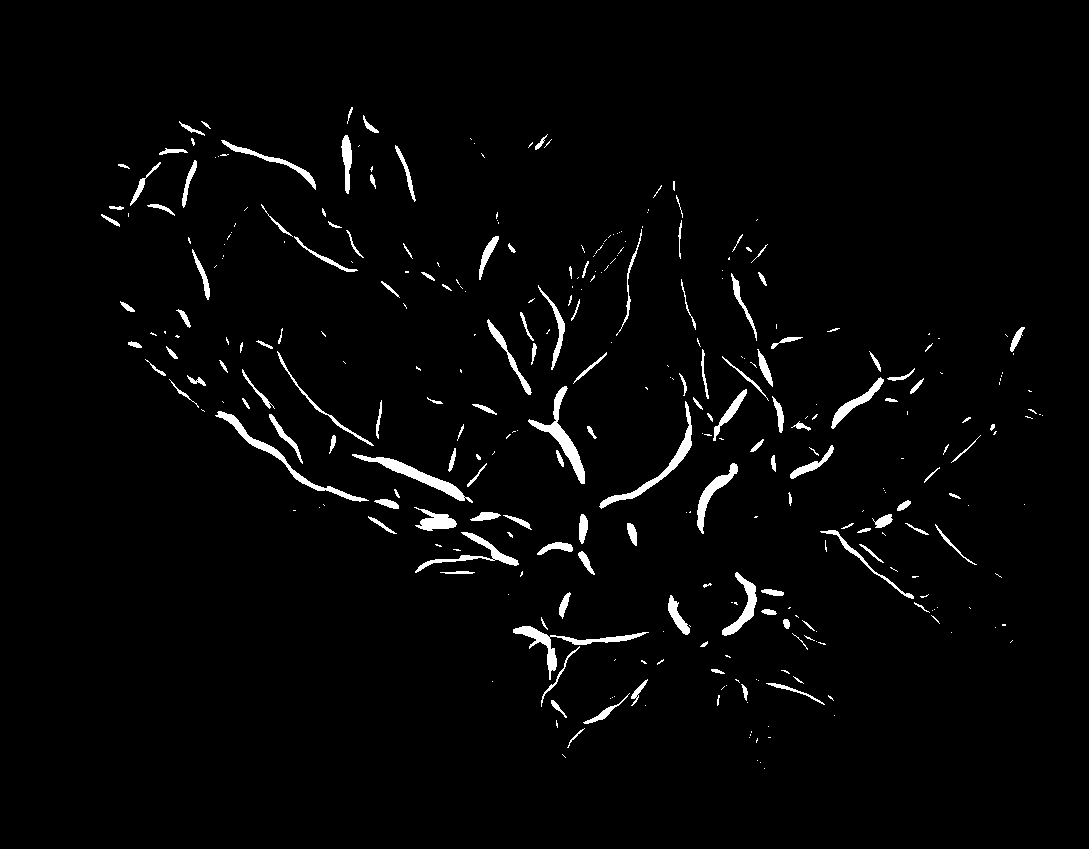
\includegraphics[width=0.48\linewidth]{qthresh_demo_q95}} \;
  \subfloat{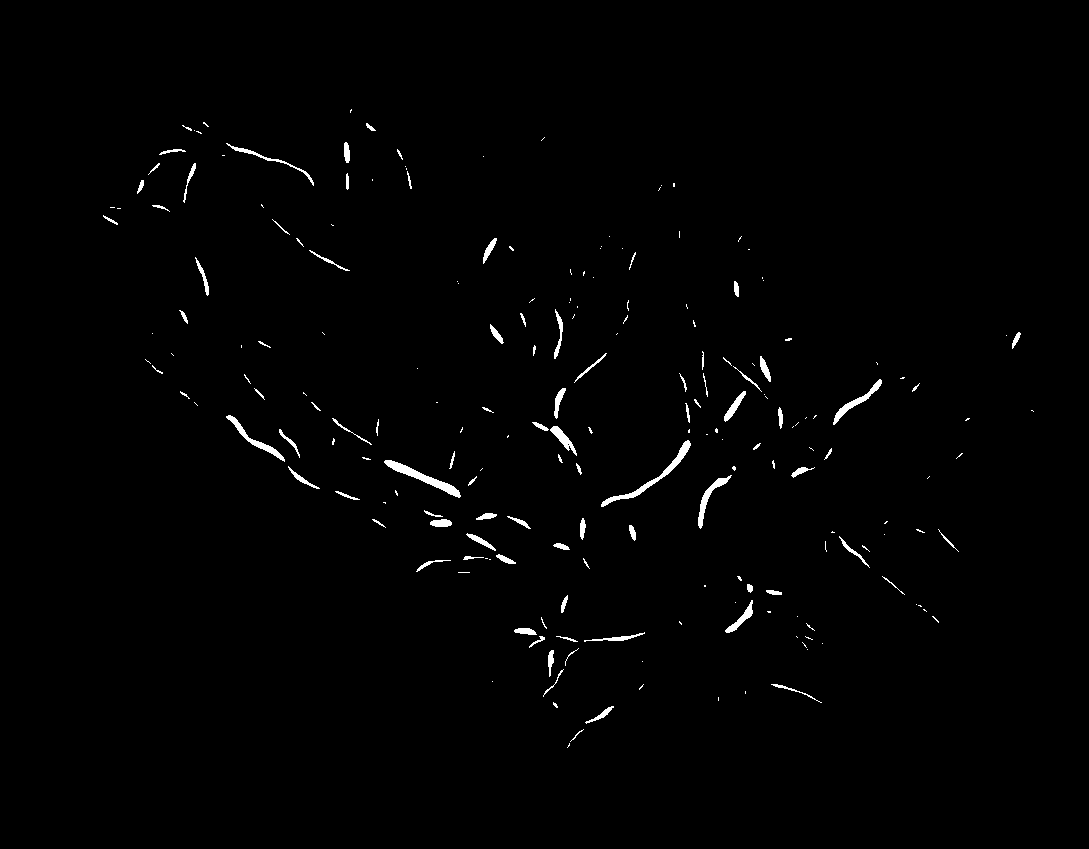
\includegraphics[width=0.48\linewidth]{qthresh_demo_q98}} \\
  \caption{Nonzero-percentile thresholding of \Vmax}.
  \label{fig:qthresh_demo}
\end{figure}

\subsection{Method C: Scale-Based Random Walker}

We observed that areas where Frangi scores are zero in well-behaved samples seem to neatly outline prominent vascular features. Following this idea, we employed a random walker segmentation \cite{Grady-Random-Walks} (which is implemented by \texttt{scikit-image}). Random walk segmentation comes about by solving a diffusion problem over a discrete array (in this case, the Frangi vesselness score itself) given starting markers. At each scale, we positively labeled pixels whose Frangi score was very high ($\Vsigma(x_0,y_0) > .4$), and negatively labeled pixels whose score was $0$ (i.e. where the leading principal eigenvalue was positive). The result of this technique is demonstrated in \cref{fig:rw-demo-scalewise} and the result (along with the original sample for comparison) is shown in \cref{fig:rw-demo-merged}.
In \cref{fig:rw-demo-scalewise}, the first column is the Frangi vesselness score at that scale, where black is a score of 0, to emphasize the difference between a score of zero and even a very small positive score, which appear in blue. The middle score are markers passed to the random walker--blue are seeds labelled with a ``1'' (where the Frangi vesselness score is 0), green is labeled ``2'' (where V > .4), and purple represents unknowns that will either assigned either label. In the last column, the result of the random walker is given--areas that have been added to the label ``2'' are shown in yellow. Although the result of random walker segmentation is technically a binary matrix, we still show the original seeds of label 2 in green for easier comparison. Similarly, the purple in the right column has actually been labeled ``1'' for non-vascular, but is left in its original color to emphasize what was assigned background. In \cref{fig:rw-demo-merged} we show the original image and the result of merging all positively marked pixels at each scale. Black means the pixel was unmatched, while increasing colors of blue (larger scales) to white (smaller scales) indicate the smallest scale from which a pixel was marked after the random walker technique. \vtodo{Do I need to over this in math methods section?} Though we shall set up the multiscale method slightly differently in \cref{ch:results-analysis}, we used a Frangi anisotropy coefficient of $\beta=0.35$ , and 12 scales logarithmically spaced from $\sigma_1 = 2^{-1.5} $ to $\sigma_{12} = 2^{3.5}$ to generate these figures. There is a parameter for the random walker algorithm (unfortunately also called $\beta$) which serves as a diffusion penalization coefficient (larger values making diffusion over the image less likely). We used \texttt{scikit-image}'s default value of 130. 

\begin{figure}[p] \centering
  \subfloat{
    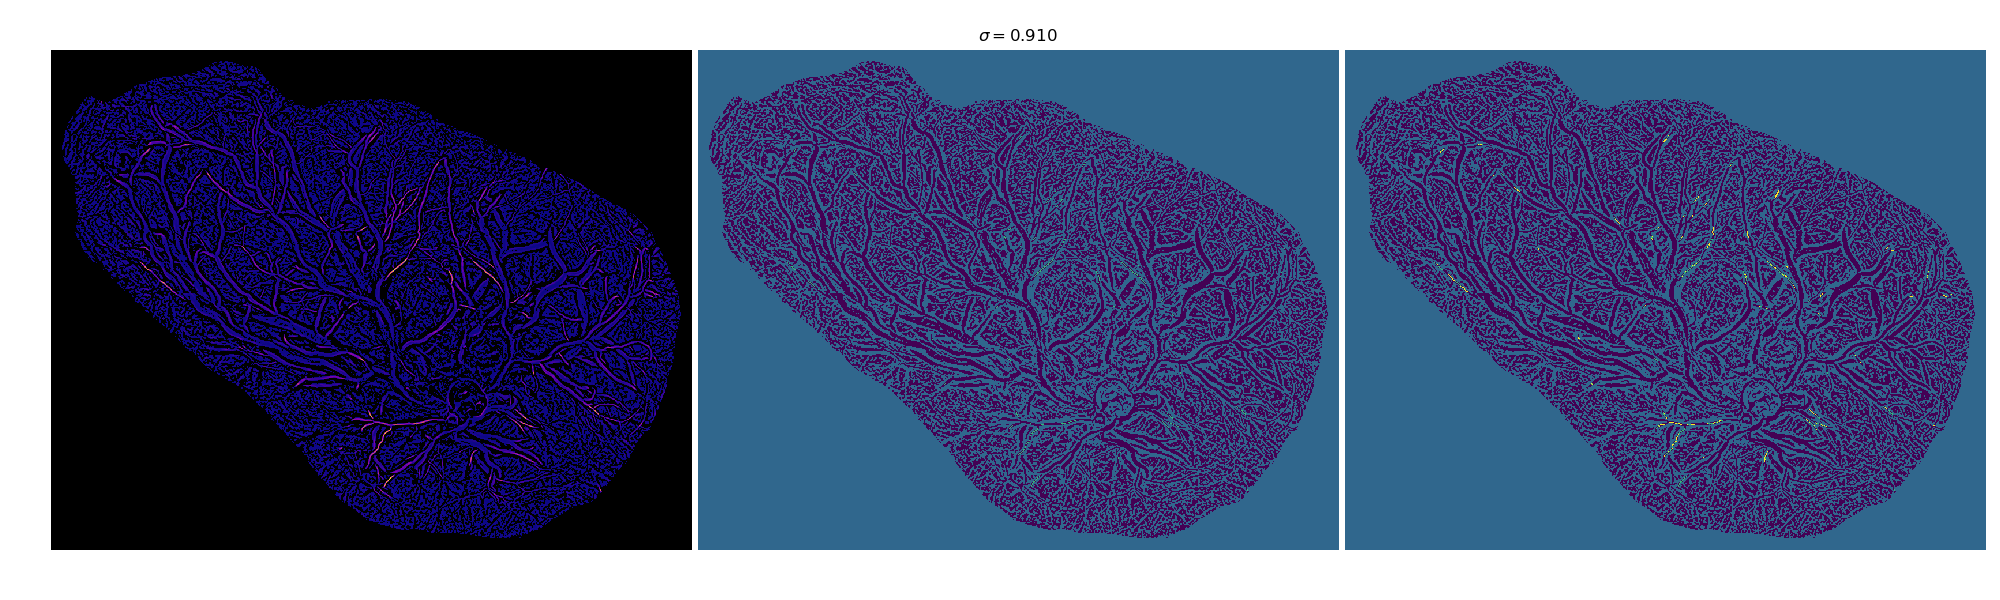
\includegraphics[width=\textwidth]{rw_demo_scale_03}
  }\\[-0.5cm]
  \subfloat{
    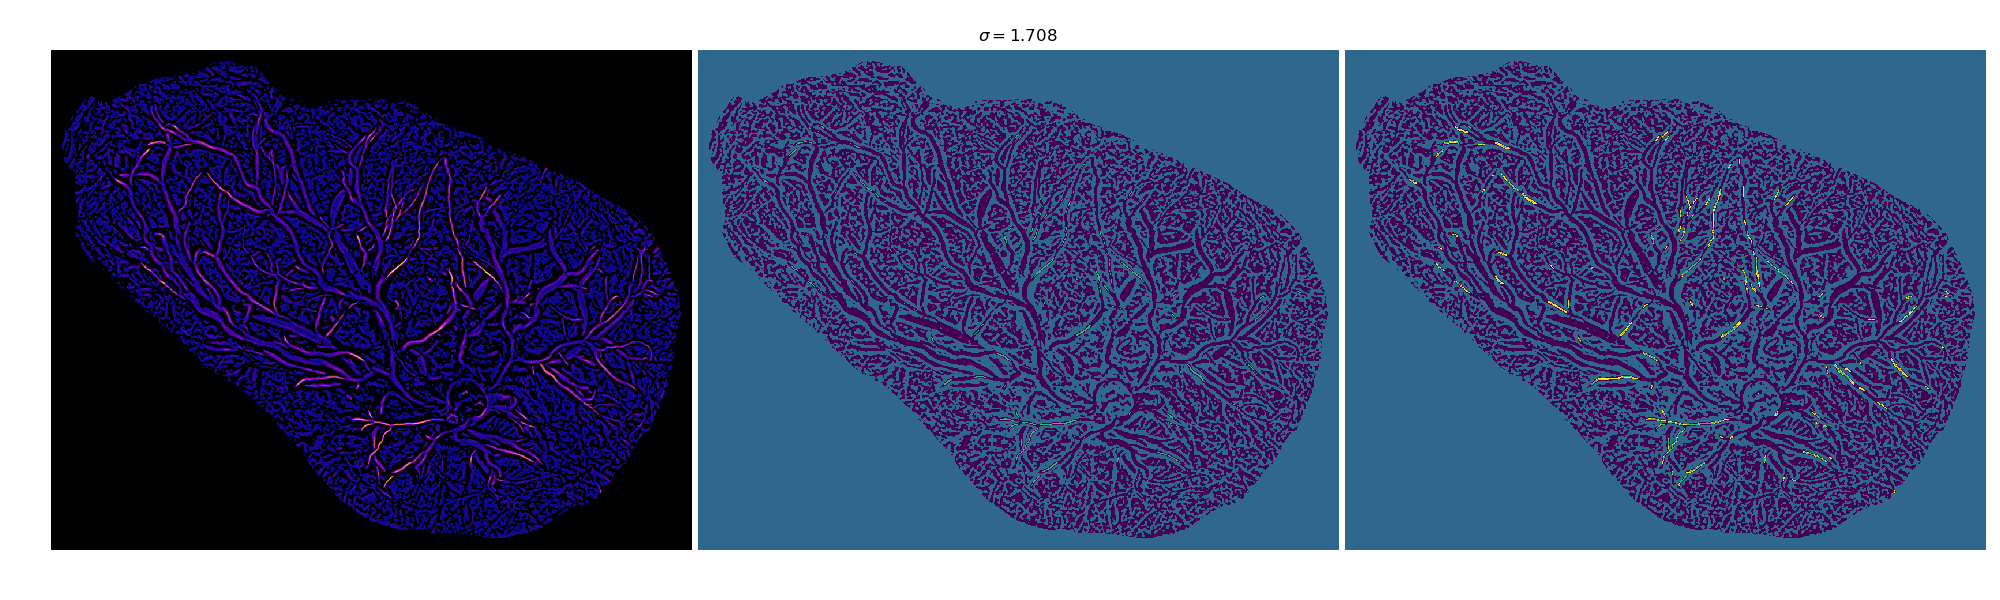
\includegraphics[width=\textwidth]{rw_demo_scale_05}
  }\\[-0.5cm]
  \subfloat{
    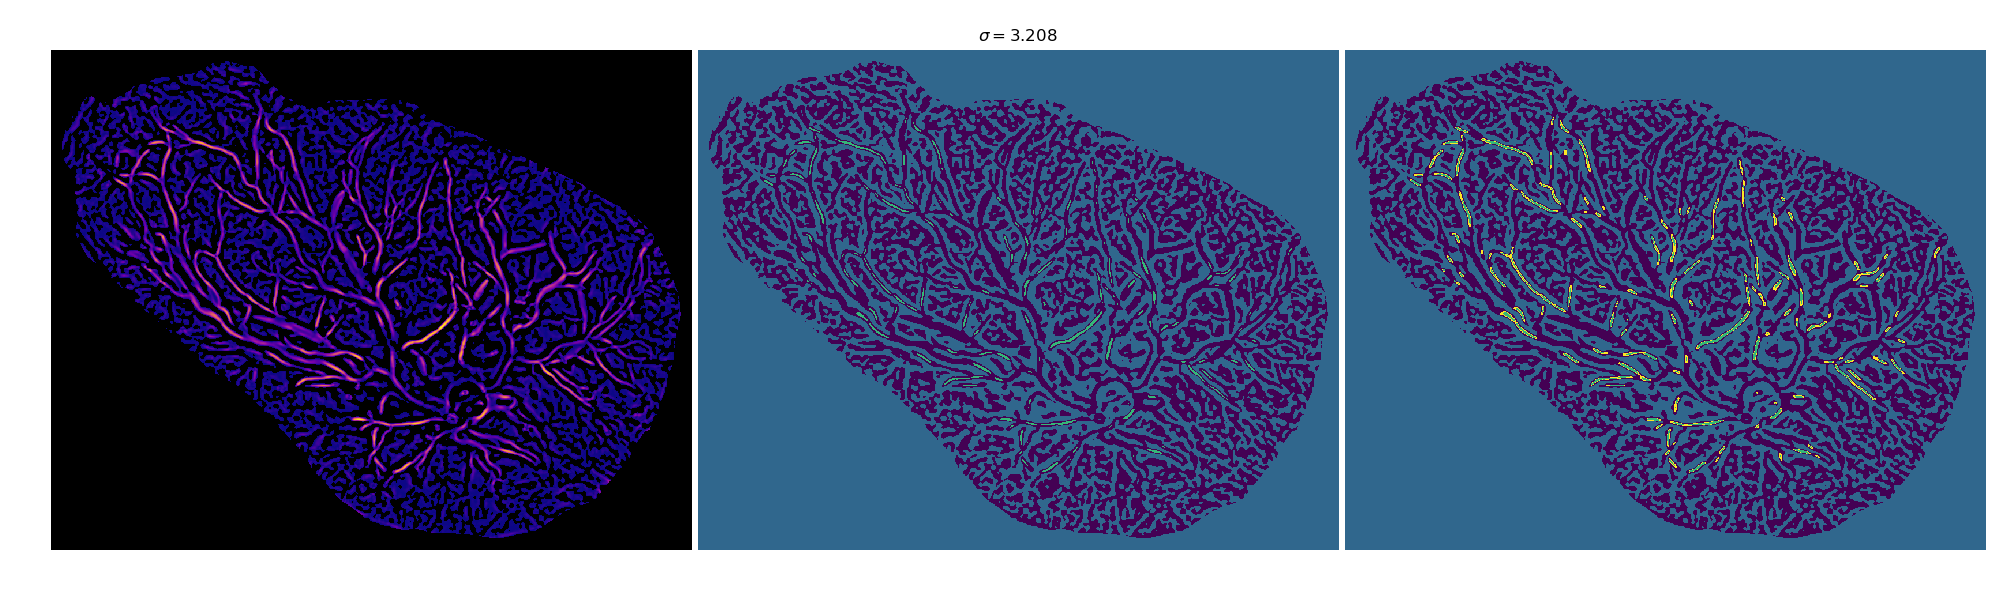
\includegraphics[width=\textwidth]{rw_demo_scale_07}
  }\\[-0.5cm]
  \subfloat{
    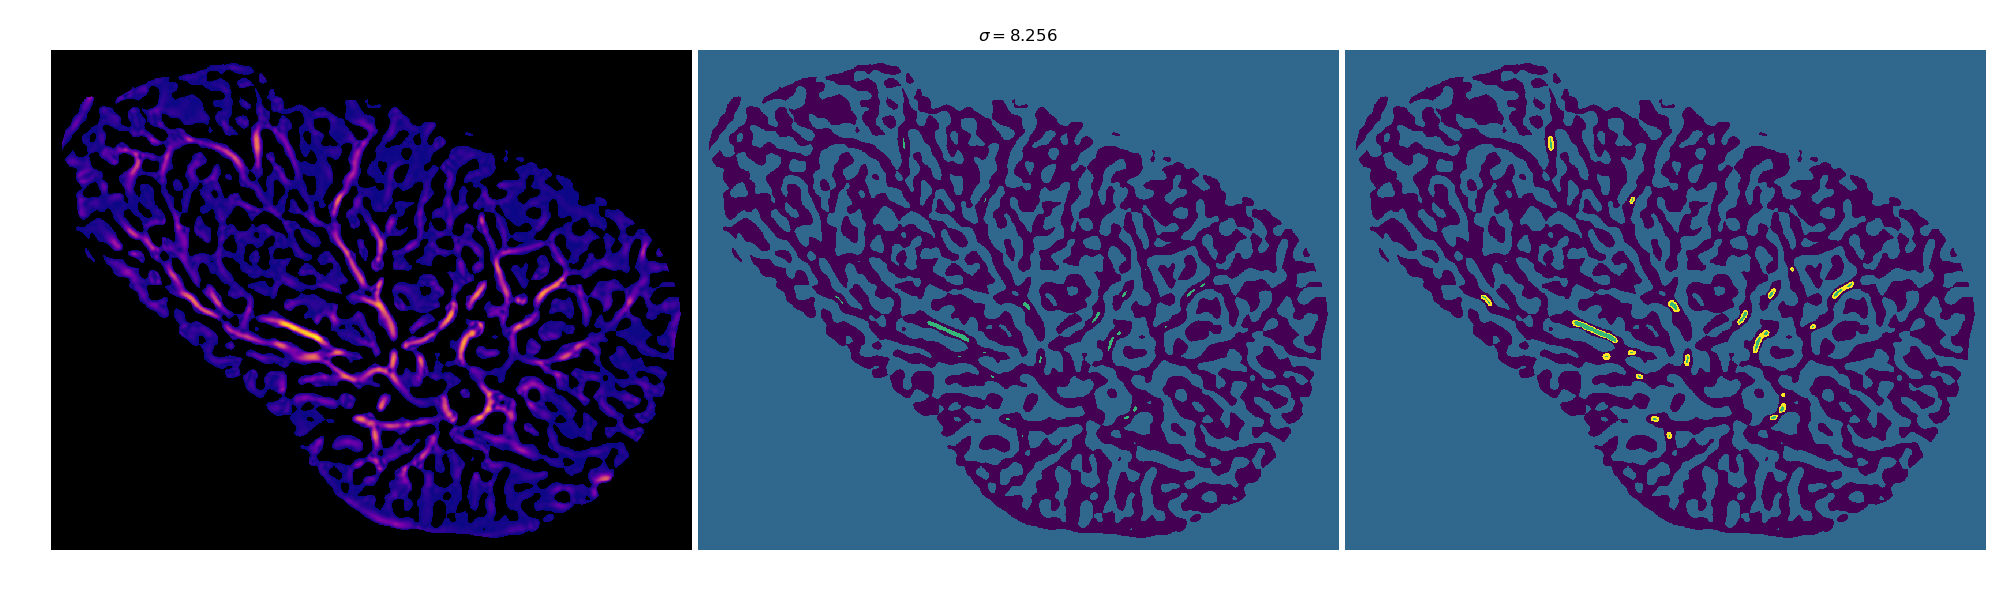
\includegraphics[width=\textwidth]{rw_demo_scale_10}
  }
  \caption{Scale-wise random walker segmentation (select scales)}
  \label{fig:rw-demo-scalewise}
\end{figure}


\begin{figure} \centering
  \subfloat{
    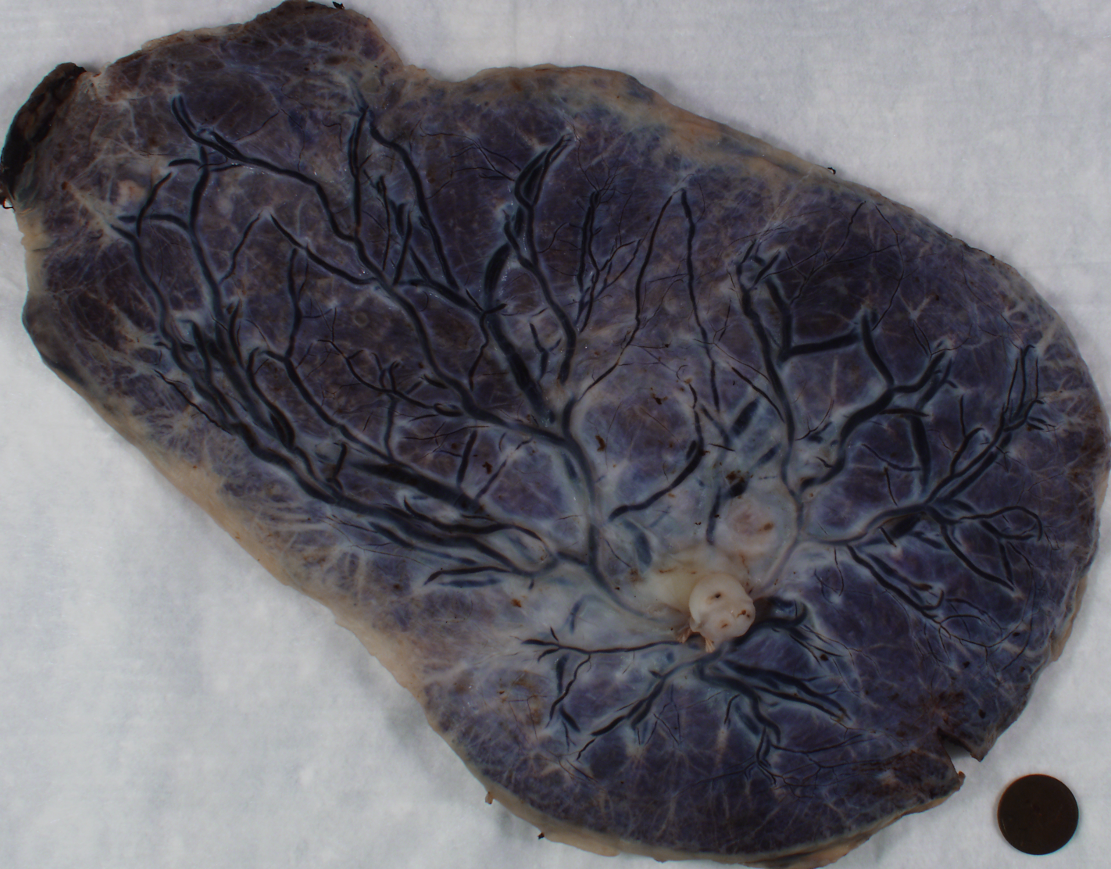
\includegraphics[height=0.3\textheight]{rw_demo_base}
  }\\
  \subfloat{
    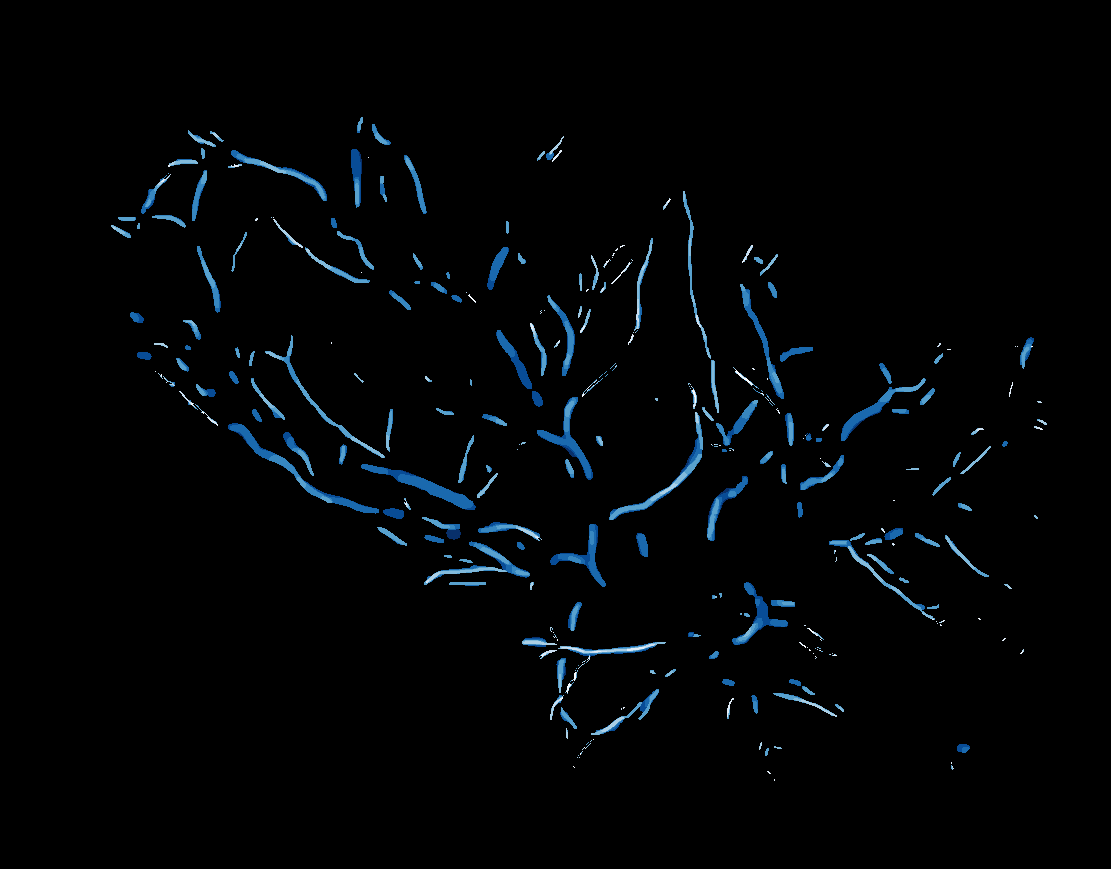
\includegraphics[height=0.3\textheight]{rw_demo_labels}
  }
  \caption{Random walker segmentation (result and sample)}
  \label{fig:rw-demo-merged}
\end{figure}

%\subsection{Method D: Scale Based Sieving}
%
%Our final approach seeks to include not only pixels at each scale that pass a high threshold, but also adjacent pixels at that scale that pass a lower threshold. We proceed as follows. At each scale, take a low threshold, then label each connected region. Then, iterate through each labeled region and add to the final approximation any labeled region that contains a pixel that passes a higher threshold.

\subsection{Method D: Trough Filling}
As we discussed in \cref{sec:signed-frangi-filter}, we can simultaneously calculate the Frangi filter for light and dark curvilinear structures without any added computation time. We shown the signed result of the  Frangi filter at different scales two examples in \cref{fig:signsweep-1} and \cref{fig:signsweep-2}, we can simultaneously calculate calculate the Frangi filter response for bright curvilinear features (dark background) and dark curvilinear features (dark background). Since the Frangi filter normally throws away any response where $\lambda_2 < 0$ (if dark curvilinear features are targeted) or $\lambda_2 >0$ (if light curvilinear features are targeted), we lose no computation time at all by simply keeping both, although we must store more results. After computing the multiscale result, we can easily separate these into a positive and a negative strain, which we will denote $\VSigmapos$ and $\VSigmaneg$, and then merge each as we would with a traditional multiscale Frangi filter, giving us
\Vmaxpos and \Vmaxneg. That is, our \Vmaxpos is the same as our \Vmax in a conventional Frangi filter, and \Vmaxneg is the same result as if we had taken the Frangi filter while only looking for the opposite type (light/dark) curvilinear feature. Plotting $\Vmax$ over a scale of $[-1,1]$ demonstrates an interesting effect. Whereas the Frangi filter generally is not reliable in terms of accurately predicting widths, we \textit{can} get a sense of the width by looking at where there is a relatively strong response of opposite sign.

\begin{figure}[p] \centering
  \subfloat{		\label{fig:signsweep-1p}\includegraphics[width=\linewidth]{{{signsweep_stitch_BN2315363_plate}}}
  } \\[-0.5cm]
  \subfloat{		\label{fig:signsweep-1i}\includegraphics[width=\linewidth]{{{signsweep_stitch_BN2315363_inset}}}
  } \\[-0.5cm]
  \subfloat{		
    \label{fig:signsweep-1c}\includegraphics[width=.75\linewidth]{{{signsweep_colorbar}}}
  } \\
  
  \caption{Signed Frangi output (plate and inset) (Example 1)}
  \label{fig:signsweep-1}
\end{figure}

\begin{figure}[p] \centering
  \subfloat{		\label{fig:signsweep-2p}\includegraphics[width=\linewidth]{{{signsweep_stitch_BN5280796_plate}}}
  } \\[-0.5cm]
  \subfloat{		\label{fig:signsweep-2i}\includegraphics[width=\linewidth]{{{signsweep_stitch_BN5280796_inset}}}
  } \\[-0.5cm]
  \subfloat{		
    \label{fig:signsweep-2c}\includegraphics[width=.75\linewidth]{{{signsweep_colorbar}}}
  } \\
  \caption{Signed Frangi output (plate and inset) (Example 1)}
  \label{fig:signsweep-2}
\end{figure}
That is, at the "foot" of every trough on either side, we can see a bordering curvilinear structure of opposite sign. We perform strict Frangi filtering and separate the positive and negative components. We then perform a different threshold for each signed portion of the Frangi response--a strict one (say $\alphapos > .3$) for the conventional $\Vmax$, and a much looser one for our opposite signed $\Vmaxneg > \alphaneg = .01$. We also truncate the scales we consider for calculating $\Vmax^{(-)}$, considering only the 6 smallest scales of 20, since we empirically notice that the bordering curvilinear features are consistently narrower than the vessels themselves.

We will refer to any pixel where $\Vmaxpos > \alphapos$ as ``in the trough'' (assuming dark curvilinear features), and any pixel where $\Vmaxneg > \alphaneg$ as potentially ``on the lip'' of the trough. The process of ``trough-filling'' then proceeds as follows.  For each pixel within the trough, we iterate over disks of integer radius and dilate the pixel by a disk of that radius if that disk includes a point on the lip (where $\Vmaxneg > \alphaneg$. This allows us to extend the Frangi output from the point where it's strongest all the way to the base of the curvilinear structure, providing a much better indication of the true width of the curvilinear structure.

\begin{figure}[p] \centering
  \subfloat{		\includegraphics[width=\textwidth]{{{fig-insetBN0164923}}}
  } \\[-0.5cm]
  \subfloat{		
    \includegraphics[width=\textwidth]{{{fig-BN0164923}}}
  } \\
  \caption{Trough dilation process (plate and inset)}
  \label{fig:trough_dilation}
\end{figure}

In \cref{fig:trough_dilation} we demonstrate the process of creating a trough dilation segments. The top left is the original sample. This was a $N=20$ Frangi filter with log range from -1.5 to 3.2 and Frangi parameters $\beta=0.15$ and $\gamma=1.0$ The middle top and top right shows $\Vmax^{(+)}$ and $\Vmax^{(-)}$ respectively. The bottom then shows the two markers 
 $\Vmax^{(-)} > \alpha^{(-)} = 0.01$ (in red) and
 $\Vmax^{(+)} > \alpha^{(-)} = .3$ (in blue). We build $\Vmax^{(-)}$ only using the 6 smallest scales, since the lighter curvilinear 'lip' of the trough is of smaller radius than the radius of the trough itself.
 
 


\section{Nonfrangi Segmentation Methods}

Of course, there are many other viable methods of segmentation. We refer to \cite{anghel2018placental} for several high-performing (albeit considerably resource intensive) segmentation methods on this dataset, namely involving shearlets, Laplacian eigenmaps, and a conditional generative adversarial network.

We will be content in the present paper to simply compare our results to a relatively fast technique that is not based on differential geometry or morphology, but instead that of a global threshold on the grayscale image. Although many viable thresholding algorithms exist, we opt for an intermeans threshold, or the Ridler-Calvert or ISODATA method, as described in \cite{isodata}, which is implemented in \texttt{scikit-image} as \texttt{filters.threshold\_isodata}. This functions uses an iterative process to find the smallest threshold which is midway between the mean intensities of the high pixels and the low pixels. In other words, the optimal $\alpha_{\textrm{ISO}}$ satisfies

\begin{equation}
\alpha_{\textrm{ISO}} = \arg\min_{\alpha} \left( \frac{1}{2} \Big[
\textrm{mean}\left\{ \img(x,y) \;|\; \img(x,y) \le \alpha \right\} 
+
\textrm{mean}\left\{ \img(x,y) \;|\; \img(x,y) >   \alpha \right\}
 \Big]
 \right)
\end{equation}

Since the vascular structure in our image domain is darker than the background, we select pixels
where $\img(x,y) < \alphaiso$.



\section{Comparison of Segmentation Methods}
In our demonstration of segmentation methods across all 201 samples in our image domain, we use the preprocessing procedure described in \cref{ch:research-protocol} Our multiscale Frangi filter setup involves 20 scales spaced logarithmically from $\sigma_1 = 2^{-1.5} \approx .35$ to $\sigma_{20} = 2^{3.2} \approx 9.20$. 

We compare a higher and lower fixed threshold (METHOD A) with
$\alpha=0.3$ and $\alpha=0.2$, and scalewise percentiles of $q=95$ and $q=98$. 

We use the trough filling method with $\alphaneg=.01$ and $\alphapos=0.3$ and we use only the first 6 scales to calculate $\Vmaxneg$.


In \cref{fig:seg-montage-example}, we look at the results of our various segmentation procedures for a typical well behaved sample. We can see that there are fewer false negatives for strict parametrization than with a standard parametrization. Even though the best MCC score across the 10 demonstrated in \cref{fig:seg-montage-example} is achieved by trough filling under standard parametrization, we note that trough filling in the strict parametrization has comparatively fewer false negatives and much higher precision. The highest precision is achieved by our higher fixed threshold. Thus, we should see the high MCC score achieved by the trough filling method as a testament to the usability of a simpler threshold as a precursor to more complete segmentation methods.

In \cref{fig:scoring-boxplots} 

Across all samples, maximum precision was achieved by the higher fixed threshold of $\alpha =0.3 $ in all but 22 samples, and the trough filling method offered the best MCC in about three-fourths of the samples (51 of 201). Where the trough filling method was not most accurate, we noticed that the $q=95 $ nz-percentile method had a slightly higher 




\begin{figure}[p] \centering
  \subfloat{ 	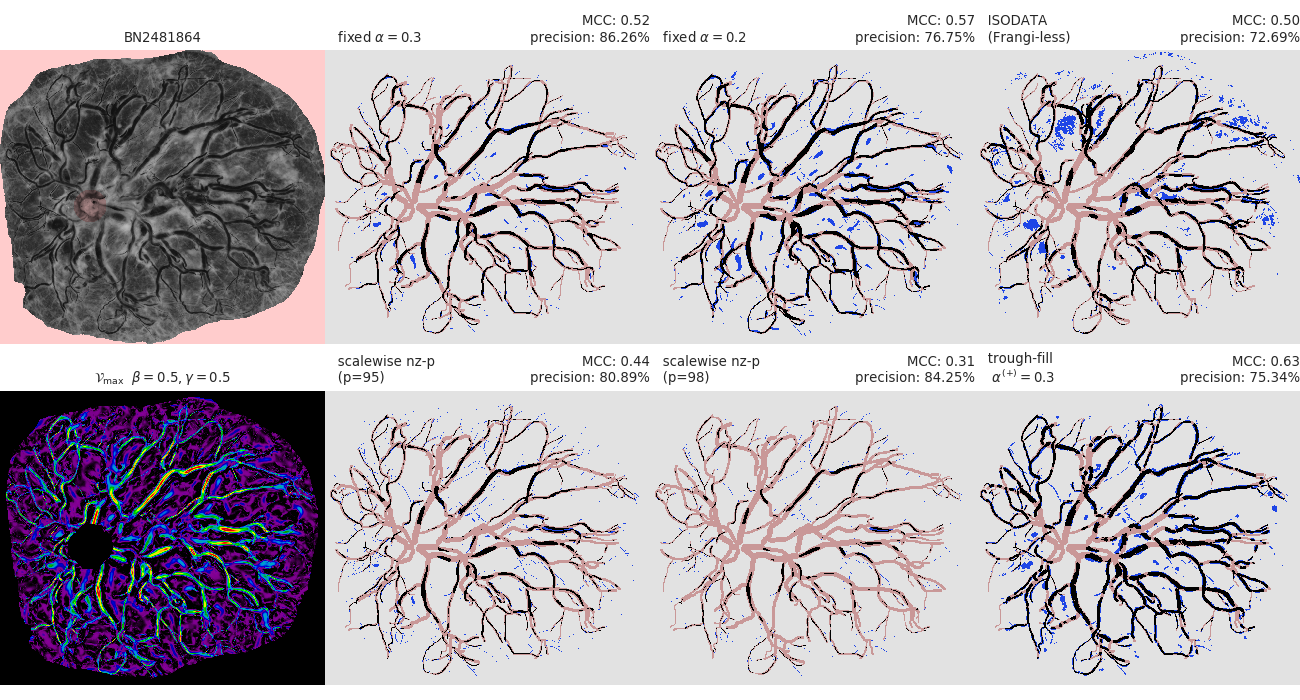
\includegraphics[width=\textwidth]{fig-BN2481864-standard-seg}} \\
  \subfloat{ 	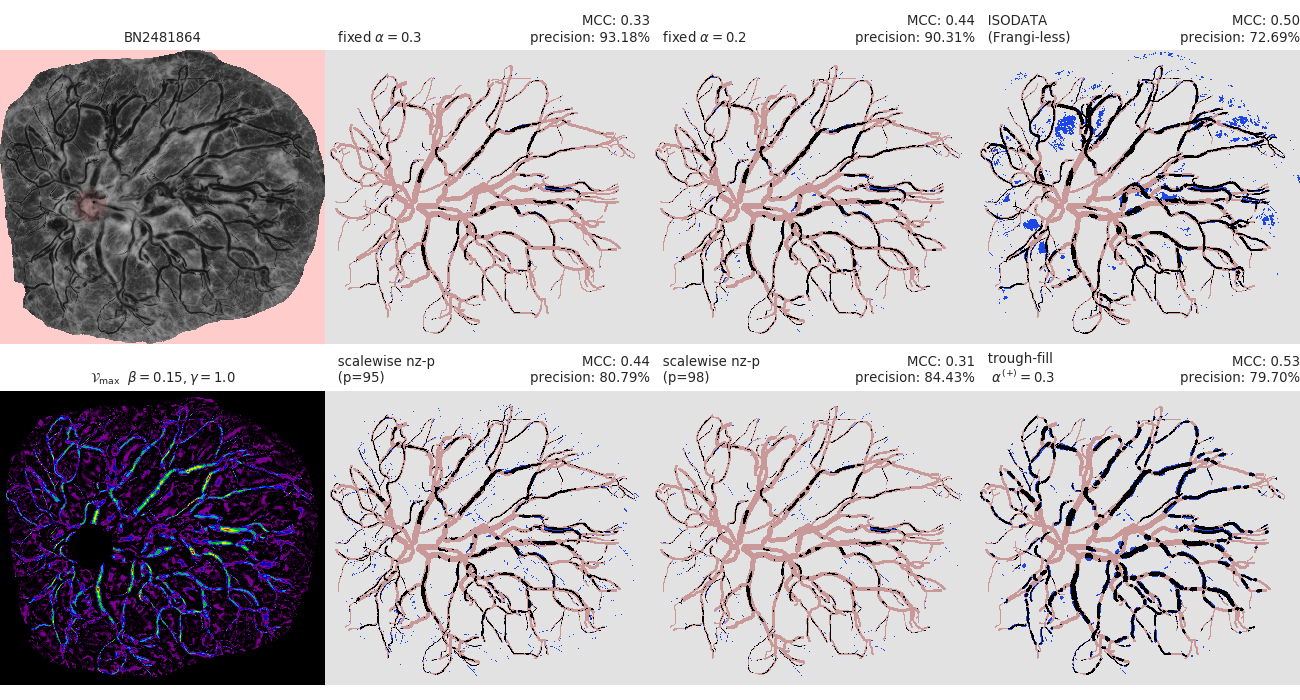
\includegraphics[width=\textwidth]{fig-BN2481864-strict-seg} }
  \caption{Confusion matrices and scores for a particular sample (standard and strict parametrization)}
	\label{fig:seg-montage-example}
\end{figure}

\begin{figure}[p] \centering
  \subfloat[standard Frangi parametrization ($\beta=0.5, \gamma=0.5$)]{  
            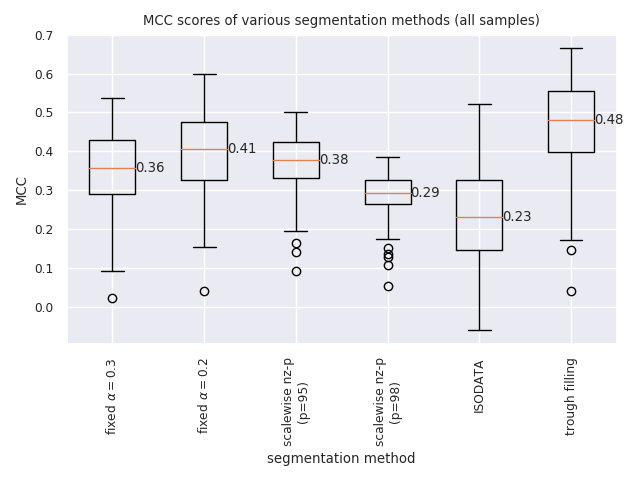
\includegraphics[width=0.5\textwidth]{all-MCC-boxplot_standard} 
            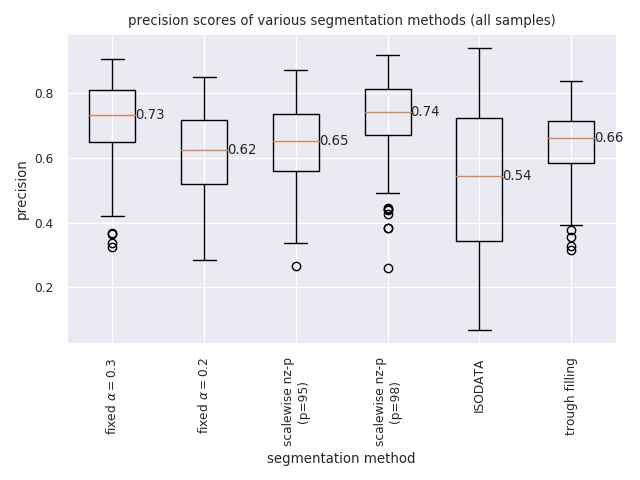
\includegraphics[width=0.5\textwidth]{all-precision-boxplot_standard} } \\
  \subfloat[semistrict Frangi parametrization ($\beta=0.15, \gamma=0.5$)]{ 
            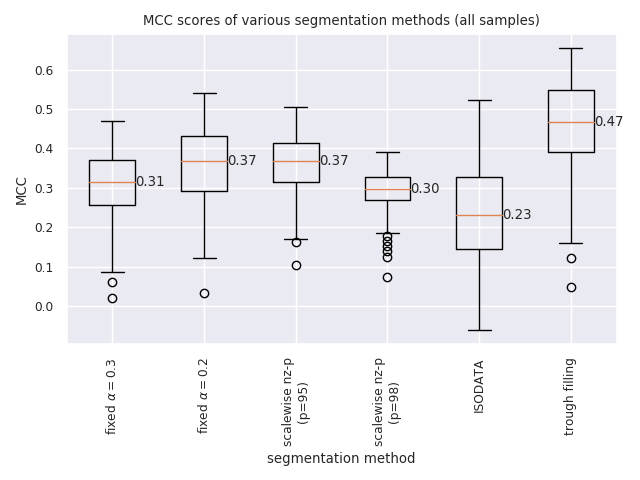
\includegraphics[width=0.5\textwidth]{all-MCC-boxplot_semistrict} 
            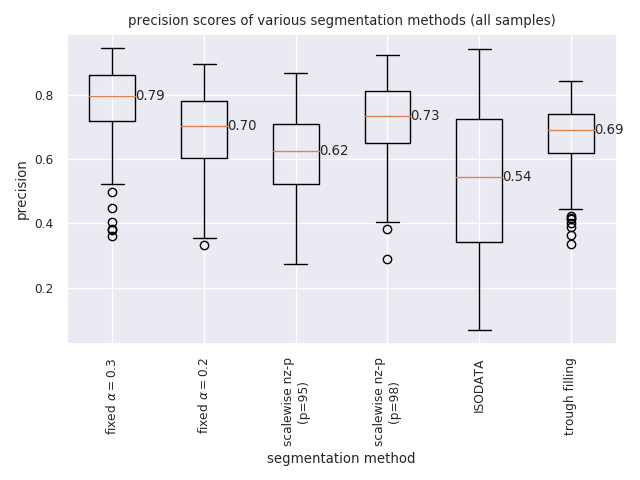
\includegraphics[width=0.5\textwidth]{all-precision-boxplot_semistrict} } \\
  \subfloat[strict Frangi parametrization ($\beta=0.15, \gamma=1.0$)]{ 
            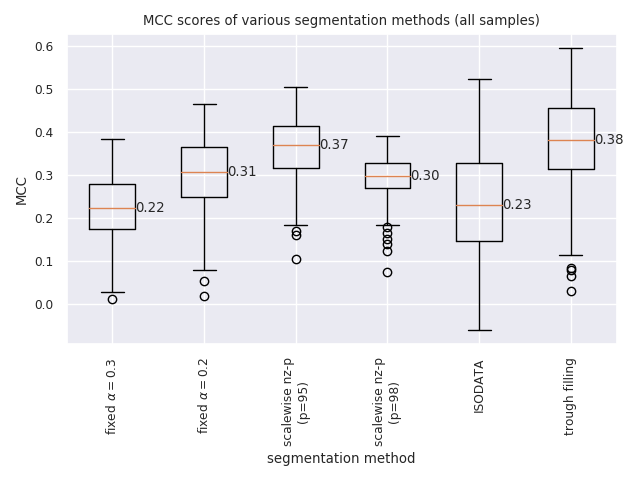
\includegraphics[width=0.5\textwidth]{all-MCC-boxplot_strict} 
            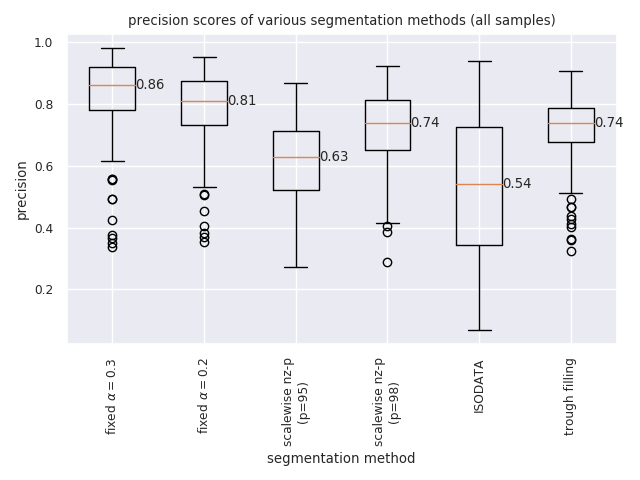
\includegraphics[width=0.5\textwidth]{all-precision-boxplot_strict} } \\
      \caption{MCC and precision of segmentation methods (201 samples)}
      \label{fig:scoring-boxplots}
\end{figure}
